%mark = star, diamond, square, otimes
%\documentclass{article}
%\usepackage{pgfplots}
%\usepackage[justification=centering]{caption}
%\pgfplotsset{compat=newest}
%\begin{document}
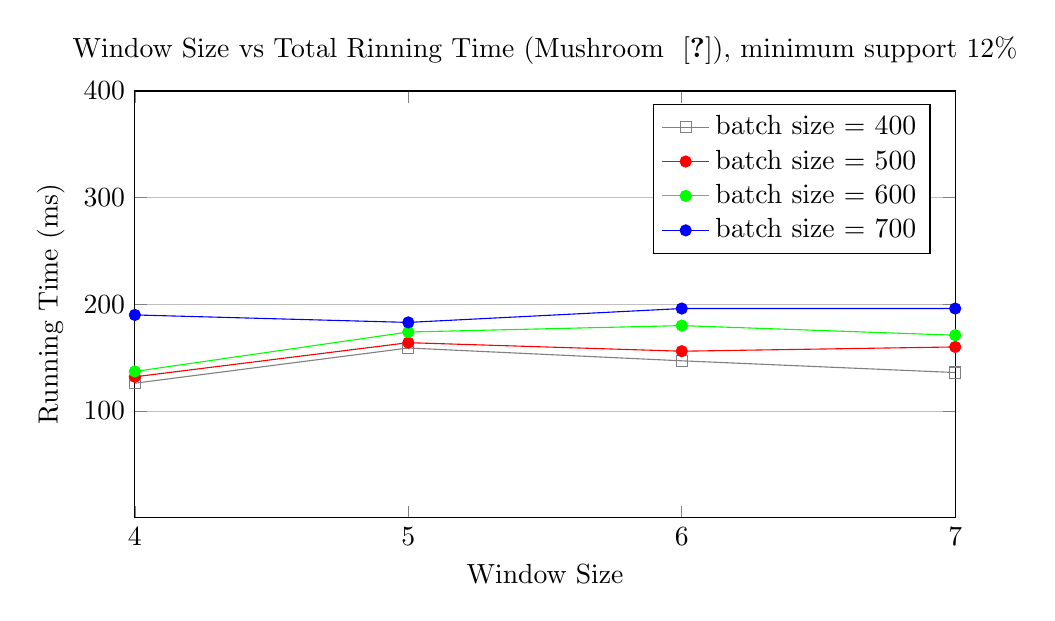
\begin{tikzpicture}
\begin{axis}[
 title={Window Size vs Total Rinning Time (Mushroom ~\cite{dataset}), minimum support 12\%},
 width=12cm,
   height=7cm,
    xlabel={Window Size},
	    ylabel={Running Time (ms)},
    xmin=4, xmax=7,
    ymin=0, ymax=400,
    xtick={4,5,6,7},
    ytick={100,200,300,400},
    legend pos=north east,
    ymajorgrids=true,
    grid style={line width=.2pt,draw=gray!50},
]
 
\addplot[
    solid,color=gray, every mark/.append style={solid, fill=gray}, mark=square
    ]
    coordinates {
			(4,126)			
			(5,159)			
			(6,147)			
			(7,136)
	};
    \addlegendentry{batch size $=$ 400}

	\addplot[
    solid,color=red, every mark/.append style={solid, fill=red}, mark=*
    ]
    coordinates {
			(4,132)			
			(5,164)			
			(6,156)			
			(7,160)
};
    \addlegendentry{batch size $=$ 500}
	

\addplot[
    solid,color=green, every mark/.append style={solid, fill=green}, mark=*
    ]
    coordinates {
			(4,137)			
			(5,174)			
			(6,180)			
			(7,171)
};
    \addlegendentry{batch size $=$ 600}
	
	
\addplot[
    solid,color=blue, every mark/.append style={solid, fill=blue}, mark=*
    ]
    coordinates {
			(4,190)			
			(5,183)			
			(6,196)			
			(7,196)
};
    \addlegendentry{batch size = 700}
\end{axis}
\end{tikzpicture}
%\end{document}